In recent years, the great demand for the Internet services (e.g. video streaming, VoIP, etc.) has led to an exponential growth in the backbone network traffic. 
Having a better knowledge about the backbone network traffic, specifically being able in predicting future traffic, thus becomes a critically important factor to perform management tasks such as traffic engineering, capacity planning and quality of service provisioning. 
For example, in the well-known Network Utility Maximization (NUM) \cite{xu2018experience}, \cite{low1999optimization} (which usually provides a bandwidth allocation or smart routing solution by solving optimization problem), the future network traffic knowledge (e.g. user demands, link usages, end-to-end latency) is used as the input. 
%These important factors are usually in the form of a traffic matrix (TM), which represents the traffic volume or latency between the origins (i.e. sources) and destinations in the network. 
However, due to the explosion of backbone network traffic as well as the complexity and dynamics of network communication behavior, modeling and estimating the future traffic in backbone networks becomes a significant challenge.

In the literature, numerous effort has been done on predicting future traffic in data centers and cellular networks.
In the traditional approaches, regression techniques (e.g., Autoregressive Integrated Moving Average (ARIMA) \cite{box2015time}) are exploited to obtain the predicted value. However, ARIMA has shown a poor performance due to two main reasons: 1) The communication behavior has become too dynamic and complicated to be modeled by a linear system. 2) ARIMA ignores the spatial relation between the traffic flows and processes the flows independently. However, the recent studies have shown that there is a strong relation between the flows, which can be utilized to improve the prediction accuracy \cite{wang2017spatiotemporal}, \cite{xie2016accurate}. 
Recently, deep learning has been widely applied to various application domains such as image/video processing, natural language recognition, etc., and achieved breakthrough results. 
In traffic analysis domain, deep learning algorithms have shown superior capability in solving the modeling and predicting non-linear time series problems. Nie et al. \cite{nie2016traffic} used Restricted Boltzmann Machine to accurately predict the future traffic volume.
Alternatively, the studies in \cite{wang2017spatiotemporal} and \cite{cao2018interactive} exploited the Convolutional Neural Network (CNN) and Long Short-Term Memory (LSTM) for capturing the spatial and temporal features. 

Unfortunately, all of the existing algorithms proposed so far require precise historical data as the input.
This requirement can be easily accomplished in the context of data centers and cellular networks since these networks are controlled through top-of-rack switches or base stations, respectively. 
However, collecting all the traffic data in backbone networks is impractical due to the complexity of network topology, the resource limitation of network devices and the high overhead of monitoring high-speed network. 
Therefore, estimating the future traffic in backbone networks suffers from the problem of missing ground-truth input where some traffic flows cannot be monitored at a particular time. 
A common approach to fill into the missing data is utilizing the data generated by the prediction model.
However, this may cause a huge degradation in the prediction's performance. 

In this paper, we address the problem of modeling and predicting the future traffic in backbone networks under the lack of historical traffic data. 
More specifically, we focus on predicting the future traffic matrices which represent the traffic volume between all the origins (i.e., sources) and the destinations in the network. 
We leverage the so-called Convolutional LSTM  (ConvLSTM, for short) network \cite{xingjian2015convolutional} (i.e., a combination of CNN and LSTM network) in extracting and modeling the spatiotemporal feature of the traffic matrix data. 
Besides that, since the prediction accuracy of the model strongly depends on the preciseness of feeding data, the most challenging problem is how to correct the feeding data so as to minimize the gap between the feeding data and the ground-truth. 
To this end, we propose two techniques. First, by constructing a backward network which processes the input in the inverse order of time, we have more information to correct the previous predicted data (which is usually imprecise) before feeding it into the model to predict the future traffic. Secondly, we construct a mechanism to sample the ground-truth at a certain rate. Specifically, by comparing the trend and the error in the historical prediction of each flow, we design a formula to determine which flows should be monitored at the next timestep. By doing so, we can balance between the monitoring overhead (in terms of flow monitoring rate) and the prediction accuracy. 
The contribution of this paper can be summarized as follows:
\begin{itemize}
\item To our best knowledge, we are the first one considering the problem of predicting future traffic in backbone networks where the historical data may be missed. Our approach is different from existing deep learning approaches in time series prediction where the model is fed with only the ground-truth input.
\item We exploit the ConvLSTM in handling the spatiotemporal of the traffic matrices in backbone networks and construct a model which combines the forward and backward ConvLSTM networks. This model is able to correct the input data to improve the accuracy of the future traffic prediction. Moreover, we also design a formula to determine which flows should be measured in the future.
\item We evaluate the performance of our proposed algorithms by conducting extensive experiments on real backbone network traffic dataset and comparing the results with state-of-the-art approaches.
\end{itemize}
The rest of the paper is organized as follows: we first introduce the problem of traffic prediction under the lack of precise input data and give a brief introduction about LSTM and ConvLSTM network in Section 2. Section 3 presents the motivation and the details of our proposed algorithms for correcting the input data and determining the monitored flow set. Section 4 shows extensive experimental results. We present some related works in Section 5 and conclude the paper in Section 6.
% \begin{figure} [bt]
% \centering
% 	\subfigure[Local minimum problem.\label{fig:intro_1}]{
% 	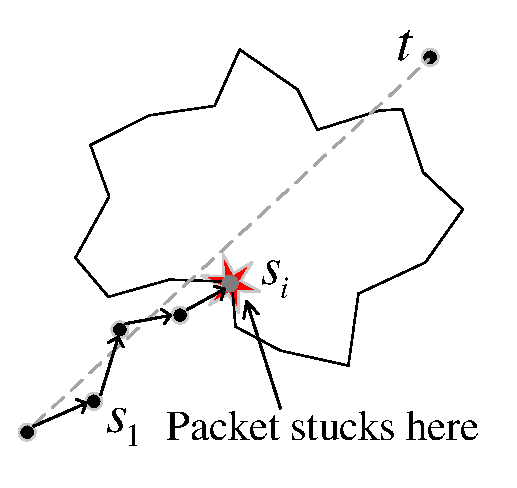
\includegraphics[width=0.35\columnwidth]{./intro_figs/intro_1.eps}
% 	}
% 	\hfill
% 	\subfigure[Congestion around the hole boundary.\label{fig:intro_2}]{
% 	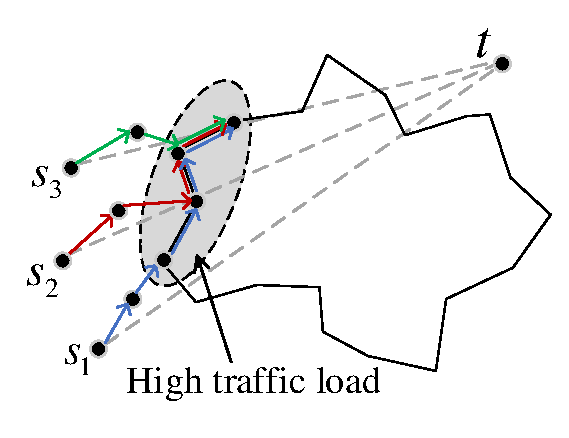
\includegraphics[width=0.4\columnwidth]{./intro_figs/intro_2.eps}
% 	}
% 	\caption{Illustrations of two serious problems that the existing protocols may encounter.}
% 	\label{fig:intro}
% \end{figure}
%
%\begin{figure*}[bt]
%    \centering
%    \begin{subfigure}[t]{0.45\textwidth}
%        \centering
%        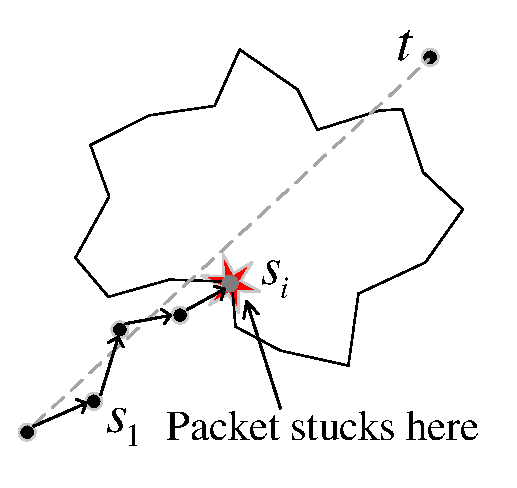
\includegraphics[width=1\columnwidth]{./intro_figs/intro_1.eps}
%        \caption{Local minimum phenomenon where the packets are stopped at the hole boundary.}
%    \end{subfigure}
%    \begin{subfigure}[t]{0.45\textwidth}
%        \centering
%        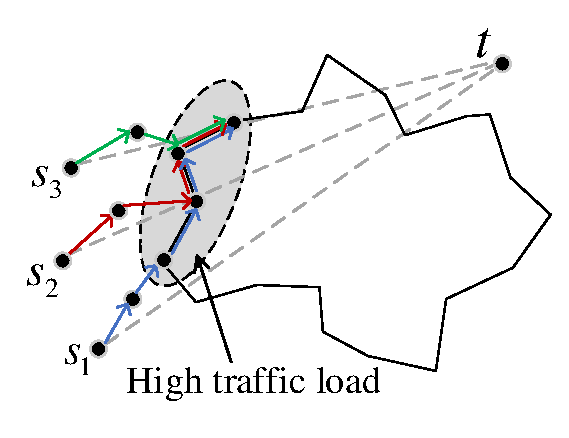
\includegraphics[width=1\columnwidth]{./intro_figs/intro_2.eps}
%        \caption{The nodes surrounding the hole boundary are imposed a heavy traffic load.}
%    \end{subfigure}
%    \caption{Illustration of two serious problems that the existing protocols may encounter.}
%\end{figure*}


